\documentclass[a4paper,12pt]{article}
\usepackage[utf8]{inputenc}

\usepackage[utf8]{inputenc}
\usepackage[T2A]{fontenc}
\usepackage[english,russian]{babel}
\usepackage{amsthm}
\usepackage{amsmath}
\usepackage{amssymb}
\usepackage{tikz}
\usepackage{textcomp}
\usepackage{marvosym}
\usepackage{ esint }
\usepackage{mathtext}
\usepackage{siunitx} % Required for alignment
\usepackage{subfigure}
\usepackage{multirow}
\usepackage{rotating}
\usepackage{afterpage}
\usepackage[arrowdel]{physics}
\usepackage{booktabs}
\setlength{\topmargin}{-0.5in}
\setlength{\textheight}{9.1in}
\setlength{\oddsidemargin}{-0.4in}
\setlength{\evensidemargin}{-0.4in}
\setlength{\textwidth}{7in}
\setlength{\parindent}{0ex}
\setlength{\parskip}{1ex}
\newcommand{\ndiv}{\hspace{-4pt}\not|\hspace{2pt}}
\usepackage{floatrow,graphicx,calc}
\usepackage{float}
\usepackage[export]{adjustbox}
\usepackage{wrapfig}
\usepackage{pgfplots}
\usepackage{caption}
\pgfplotsset{compat=1.16}
\graphicspath{ {./images/} }
\RequirePackage{caption}
\DeclareCaptionLabelSeparator{defffis}{ — }
\captionsetup{justification=centering,labelsep=defffis}
\usepackage{caption} \captionsetup[table]{labelsep=endash,justification=justified,singlelinecheck=false,font=normalsize}
\usepackage{amsfonts,mathtools}

\title{Лабораторная работа № 5.4.2\\Исследование энергетического спектра $\beta$-частиц и определение их максимальной энергии при помощи магнитного спектрометра}
\author{Илья Прамский}
\date{Октябрь 2024}

\begin{document}
\maketitle
\newpage
\section{Теоретическая справка}
Электронный $\beta$-распад:
\begin{equation}
^A_ZX \rightarrow ^A_{Z+1}X + e^- + \widetilde{\nu}
\end{equation}
Величина $W(p_e)$ является плотностью вероятности. Распределение электронов по энергии может быть вычислено теоретически. Для разрешенных переходов вероятность $\beta$-распада просто попрорциональна сатистическому весу.
	\begin{equation}
		\label{eq:W}
		W(p_e)dp_e \propto p_e^2(T_m-T_e)^2 dp_e.
	\end{equation}
	Кинетическая энергия электрона и его импульс связаны друг с другом обычной формулой:
	\begin{equation*}
		T = \sqrt{(p_ec)^2+(m_ec^2)^2}-m_ec^2
	\end{equation*}
	Выражение (2) приводит к спектру, имеющему вид широкого колокола. Кривая плавно отходит от нуля и стольже плавно, по параболе, касается оси абсцисс в области максимального импульса электронов.
	
\section{Экспериментальная установка}
	Блок-схема установки для изучения $\beta$-спектров изображена на схеме слева.
	
	\begin{figure}[h!]
				{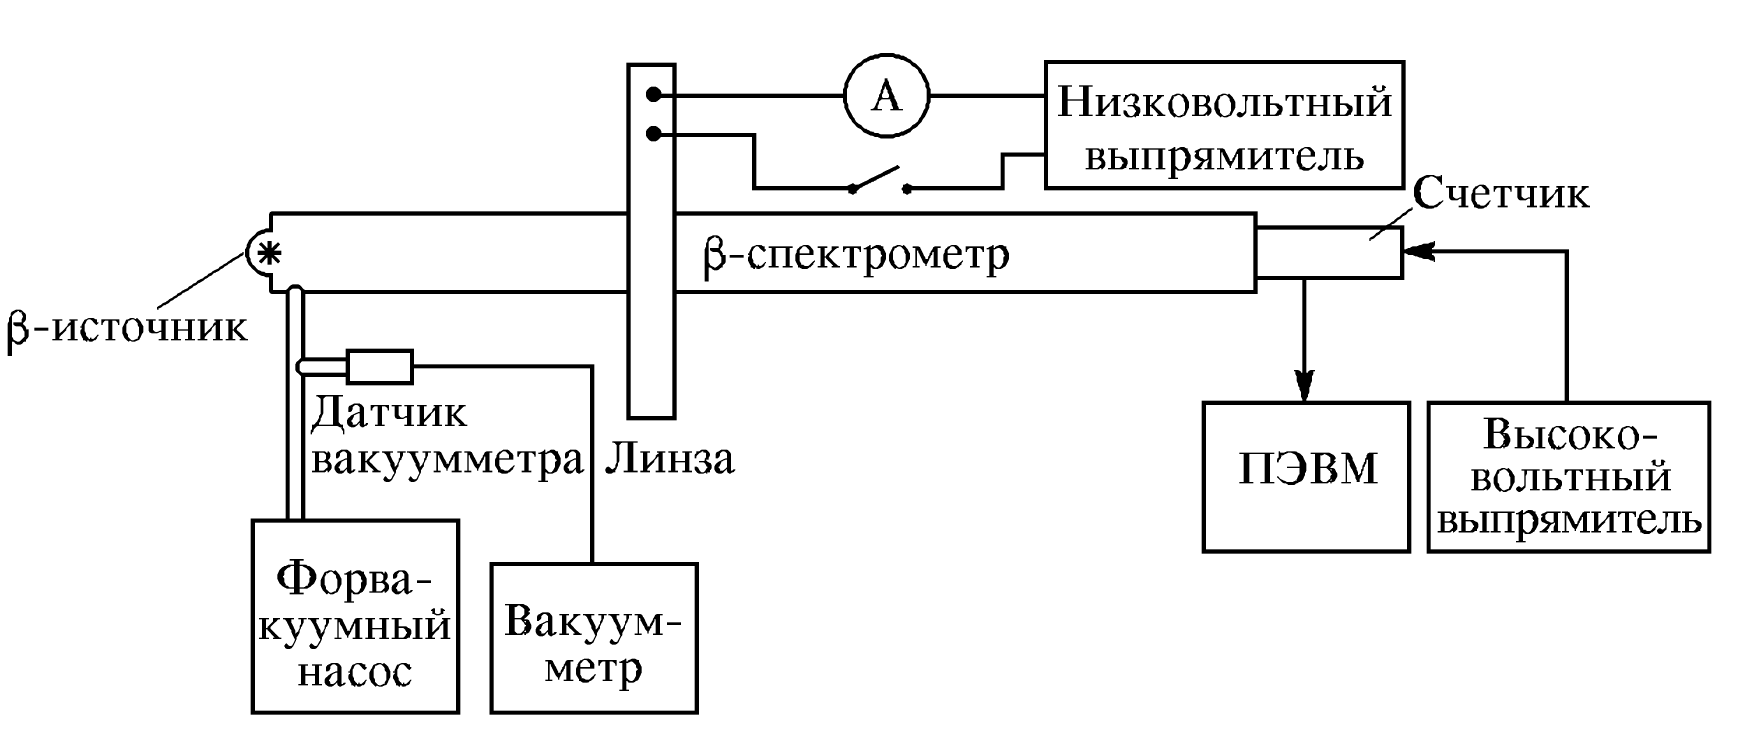
\includegraphics[width=8cm,height=4cm]{shema.png}{\label{pic1}}}
				{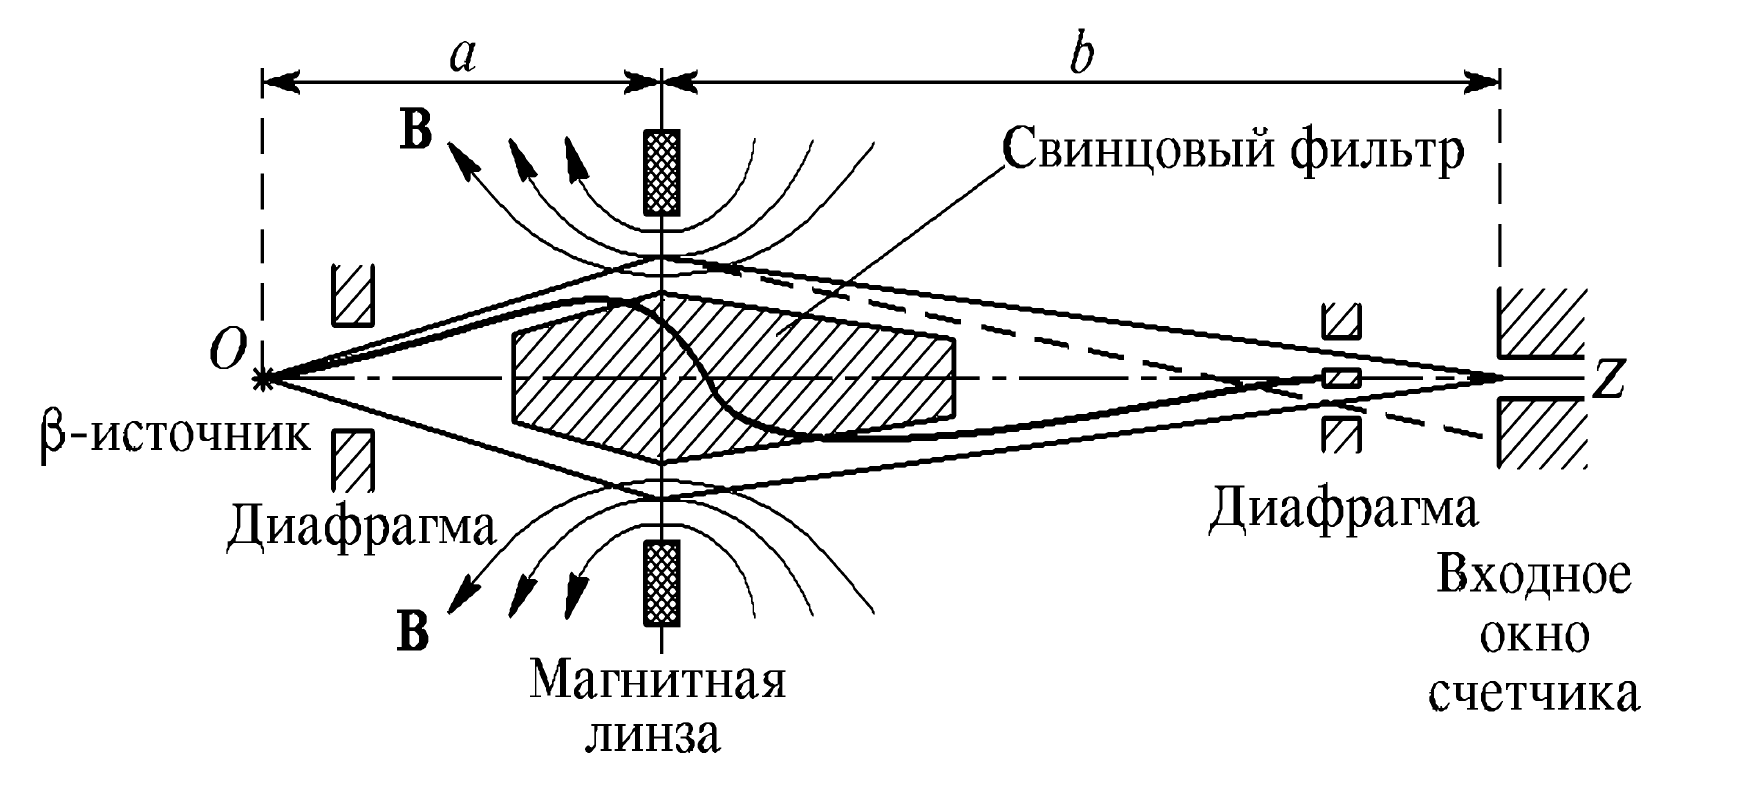
\includegraphics[width=8cm,height=4cm]{ustanovka.png}{\label{pic2}}}         
		{\caption*{Экспериментальная установка.}}
	\end{figure}

	Энергию $\beta$-частиц определяют с помощью $\beta$-спектрометров(схема справа). импульс сфокусированных электронов пропорционален величине тока:
	\begin{equation}
		\label{eq:pkI}
		p_e = kI.
	\end{equation}

	Cвязь между числом частиц, регистрируемых установкой, и функцией $W(p_e)$ выражается формулой:
	\begin{equation*}
		N(p_e) \propto W(p_e)p_e,
	\end{equation*}
	откуда
	\begin{equation}
		\label{eq:fermi}
		\frac{\sqrt{N}}{p_e^{3/2}} \propto T_m - T
	\end{equation}
\newpage
\section{Ход работы}
Полученные в результате эксперимента значения представлены на фото:
\begin{figure}[H]
\centering
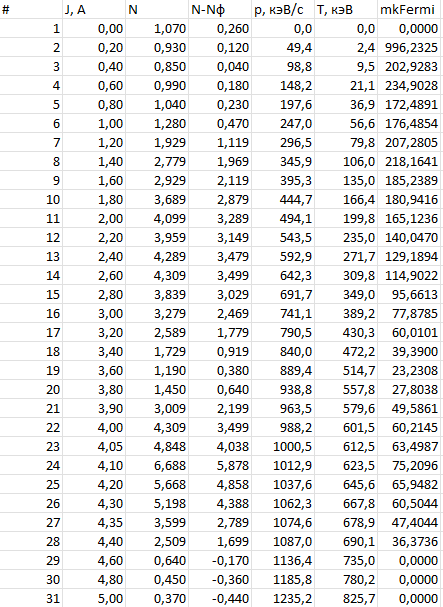
\includegraphics[scale=1]{tabl1.png}
\end{figure}
Графики зависимости N-Nф от J,p,T:
\begin{figure}[H]
\centering
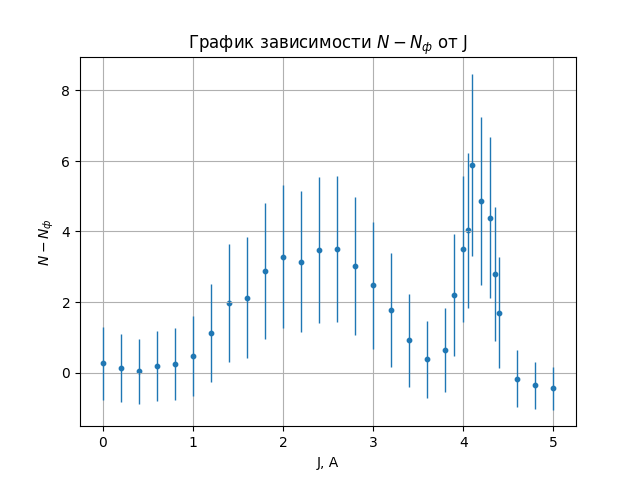
\includegraphics[scale=0.7]{graph1.png}
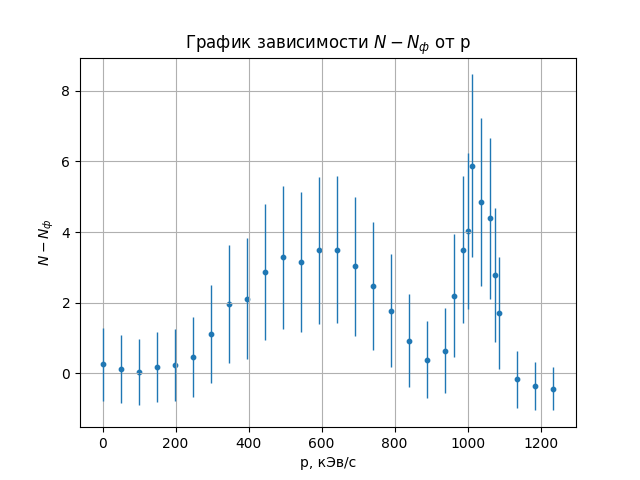
\includegraphics[scale=0.7]{graph2.png}
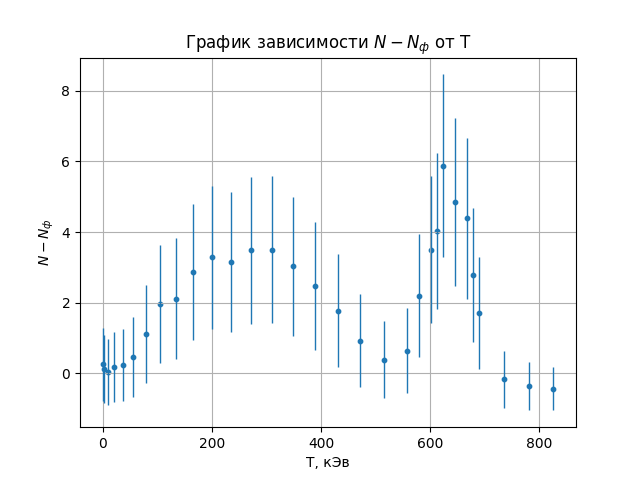
\includegraphics[scale=0.7]{graph3.png}
\end{figure}

График Ферми-Кюри:
		\begin{figure}[H]
			\begin{floatrow}
			{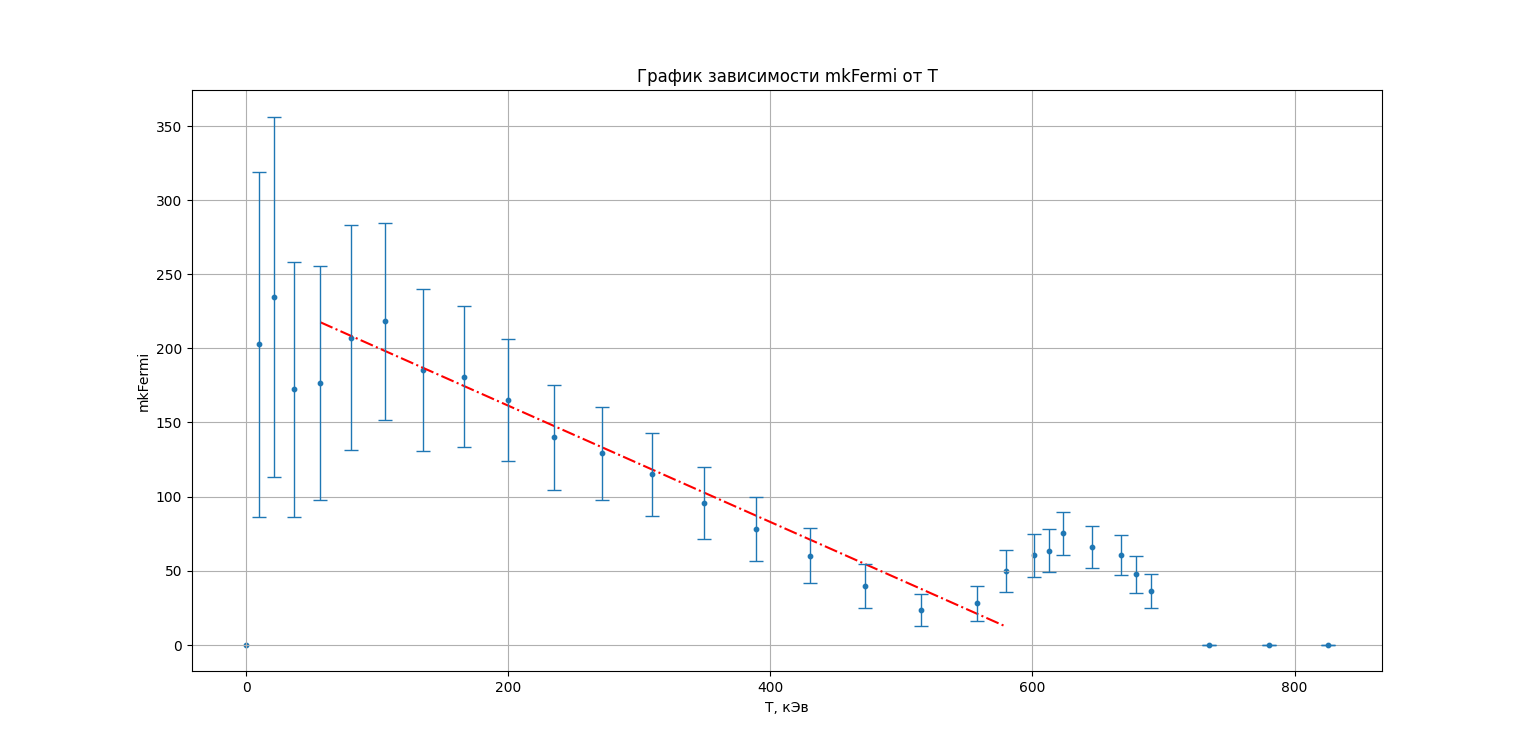
\includegraphics[width=20cm,height=12cm, left]{graph4.png}}   
			\end{floatrow}
		\end{figure}
	
Определим по нему значение $T_{max}$.
$k = -0,39 \pm 0,02$ \\
$b = 240 \pm 8$ \\
\[T_{max} = -\frac{b}{k} = 620 \pm 40 \text{кэВ}\]
\section{Вывод}
В ходе лабораторной работы с помощью магнитного спектрометра был исследован энергетический спектр $\beta$-частиц при распаде ядер $^{137}$Cs. При помощи графика Ферми-Кюри была также определена максимальная энергия $T_{max} = 620 \pm 40$ кэВ вылетающих электронов при $\beta$-распаде ядря $^{137}$Cs. Истинное же значение равно $T_{max} = 624$ кэВ.
\end{document}